\documentclass[
  xcolor={svgnames},
  hyperref={colorlinks,citecolor=DeepPink4,linkcolor=DarkRed,urlcolor=DarkBlue},
  UTF8
  ]{beamer}
\usepackage{amsmath}
\usepackage{amssymb}
\usepackage{amsfonts}
\usepackage[utf8]{inputenc}
\usepackage{graphicx}
\usepackage{hyperref}
\usepackage{xcolor}
\usepackage{wasysym}
\usepackage{listings}
\usepackage{tikz}
\usepackage[normalem]{ulem}
\usepackage{textcomp}
\usepackage{verbatim}
\usepackage[T1]{fontenc}
\usepackage{lmodern}
\usepackage[framemethod=tikz]{mdframed}
\usepackage{upquote}

\usetikzlibrary{shapes.callouts,shadows, calc}

\tikzset{note/.style={rectangle callout, rounded corners,fill=gray!20,drop shadow,font=\footnotesize}}    
\newcommand{\tikzmark}[1]{\tikz[overlay,remember picture] \node (#1) {};}    

\newcounter{image}
\setcounter{image}{1}

\makeatletter
\newenvironment{btHighlight}[1][]
{\begingroup\tikzset{bt@Highlight@par/.style={#1}}\begin{lrbox}{\@tempboxa}}
{\end{lrbox}\bt@HL@box[bt@Highlight@par]{\@tempboxa}\endgroup}

\newcommand\btHL[1][]{%
  \begin{btHighlight}[#1]\bgroup\aftergroup\bt@HL@endenv%
}
\def\bt@HL@endenv{%
  \end{btHighlight}%   
  \egroup
}
\newcommand{\bt@HL@box}[2][]{%
  \tikz[#1]{%
    \pgfpathrectangle{\pgfpoint{0pt}{0pt}}{\pgfpoint{\wd #2}{\ht #2}}%
    \pgfusepath{use as bounding box}%
    \node[anchor=base west,rounded corners, fill=green!30,outer sep=0pt,inner xsep=0.2em, inner ysep=0.1em,  #1](a\theimage){\usebox{#2}};
  }%
 \stepcounter{image}
}
\makeatother

\usetheme{Warsaw}
\usecolortheme{lily}
\setbeamercovered{transparent}
\setbeamertemplate{headline}{
  \begin{beamercolorbox}{section in head/foot}
    \vskip2pt\insertnavigation{\paperwidth}\vskip2pt
  \end{beamercolorbox}
}

\setbeamertemplate{footline}{
}

\author{
  {\tiny Tony Morris\\}
}

\xdefinecolor{darkgreen}{rgb}{0,0.35,0}
\lstset{
  tabsize=2,
  basicstyle=\ttfamily,
  moredelim=**[is][\btHL]{`}{`}
}
\lstdefinelanguage{java}{
  morekeywords={abstract,assert,boolean,break%
    byte,case,catch,char,class,const,continue%
    default,do,double,else,enum,extends,false%
    final,finally,float,for,goto,if,implements%
    import,instanceof,int,interface,long,native%
    new,null,package,private,protected,public%
    return,short,static,strictfp,super,switch%
    synchronized,this,throw,throws,transient%
    true,try,void,volatile,while},
  otherkeywords={=,=>,<-,<\%,<:,>:,\#,@},
  sensitive=true,
  morecomment=[l]{//},
  morecomment=[n]{/*}{*/},
  morestring=[b]",
  morestring=[b]',
  morestring=[b]"""
}
\lstdefinelanguage{csharp}
{
  sensitive=true,
  morekeywords=[1]{
  abstract, as, base, break, case,
  catch, checked, class, const, continue,
  default, delegate, do, else, enum,
  event, explicit, extern, false,
  finally, fixed, for, foreach, goto, if,
  implicit, in, interface, internal, is,
  lock, namespace, new, null, operator,
  out, override, params, private,
  protected, public, readonly, ref,
  return, sealed, sizeof, stackalloc,
  static, struct, switch, this, throw,
  true, try, typeof, unchecked, unsafe,
  using, virtual, volatile, while, bool,
  byte, char, decimal, double, float,
  int, lock, object, sbyte, short, string,
  uint, ulong, ushort, void},
  morecomment=[l]{//},
  morecomment=[s]{/*}{*/},
  morecomment=[l][keywordstyle4]{\#},
  morestring=[b]",
  morestring=[b]',
}
\lstdefinelanguage{haskell}{
  morekeywords={class,instance,where,do,data,newtype,default,deriving,module},
  otherkeywords={<-},
  sensitive=true,
  morecomment=[l]{--},
  morecomment=[n]{\{-}{-\}}, 
  morestring=[b]",
  morestring=[b]',
  morestring=[b]"""
}
\lstdefinelanguage{python}{
 keywords={catch, def, float, lambda, in, int, null, self, str, switch, typeof},
 keywordstyle=\color{ForestGreen}\bfseries,
 ndkeywords={boolean, throw, import},
 ndkeywords={return, class, if ,elif, endif, while, do, else, True, False , catch, def},
 ndkeywordstyle=\color{red}\bfseries,
 identifierstyle=\color{black},
 sensitive=false,
 comment=[l]{\#},
 morecomment=[s]{/*}{*/},
 commentstyle=\color{purple}\ttfamily,
 stringstyle=\color{red}\ttfamily,
}
\lstdefinelanguage{scala}{
  morekeywords={abstract,case,catch,class,def,%
    do,else,extends,false,final,finally,%
    for,forSome,if,implicit,import,lazy,match,%
    new,null,object,override,package,%
    private,protected,requires,return,sealed,%
    super,this,throw,trait,true,try,%
    type,val,var,while,with,yield},
  otherkeywords={=,=>,<-,<\%,<:,>:,\#,@},
  sensitive=true,
  morecomment=[l]{//},
  morecomment=[n]{/*}{*/},
  morestring=[b]",
  morestring=[b]',
  morestring=[b]"""
}
\lstdefinestyle{haskell}{
  language=haskell,
  basicstyle=\tiny\ttfamily,
  stringstyle=\color{darkgreen}\ttfamily,
  commentstyle=\color{gray}\ttfamily,
  keywordstyle=\footnotesize\color{blue}\ttfamily,
  tabsize=2,
  moredelim=**[is][\btHL]{`}{`}
}
\lstdefinestyle{java}{
  language=java,
  basicstyle=\footnotesize\ttfamily,
  stringstyle=\color{darkgreen}\ttfamily,
  commentstyle=\color{gray}\ttfamily,
  keywordstyle=\footnotesize\color{blue}\ttfamily,
  tabsize=2,
  moredelim=**[is][\btHL]{`}{`}
}
\lstdefinestyle{python}{
  language=python,
  basicstyle=\footnotesize\ttfamily,
  stringstyle=\color{darkgreen}\ttfamily,
  commentstyle=\color{gray}\ttfamily,
  keywordstyle=\footnotesize\color{blue}\ttfamily,
  tabsize=2,
  moredelim=**[is][\btHL]{`}{`}
}
\lstdefinestyle{csharp}{
  language=csharp,
  basicstyle=\tiny\ttfamily,
  stringstyle=\color{darkgreen}\ttfamily,
  commentstyle=\color{gray}\ttfamily,
  keywordstyle=\tiny\color{blue}\ttfamily,
  tabsize=2,
  moredelim=**[is][\btHL]{`}{`}
}
\lstdefinestyle{scala}{
  language=scala,
  basicstyle=\footnotesize\ttfamily,
  stringstyle=\color{darkgreen}\ttfamily,
  commentstyle=\color{gray}\ttfamily,
  keywordstyle=\footnotesize\color{blue}\ttfamily,
  tabsize=2,
  moredelim=**[is][\btHL]{`}{`}
}
% #866eaa
\definecolor{nicta-purple}{rgb}{0.5234,0.4297,0.6640}

\defbeamertemplate*{title page}{customized}[1][] {
  \centering
  \color{nicta-purple}
  \usebeamerfont{title}\inserttitle\par
  \bigskip
  \usebeamerfont{subtitle}\insertsubtitle\par
  \bigskip
  \bigskip
  \bigskip
  \bigskip
  \usebeamerfont{institute}\insertinstitute\par
  \bigskip
  \usebeamerfont{author}\insertauthor\par
  % \usebeamerfont{date}\insertdate\par
  \usebeamercolor[fg]{titlegraphic}\inserttitlegraphic
}

\logo{
\includegraphics[height=0.8cm]{image/data61-csiro.jpg}}


\setbeamercovered{transparent}

\begin{document}

\newmdenv[tikzsetting={draw=black,fill=white,fill opacity=0.7, line width=4pt},backgroundcolor=none,leftmargin=0,rightmargin=0,innertopmargin=4pt]{Conference}

\newmdenv[tikzsetting={draw=black,fill=white,fill opacity=0.7, line width=4pt},backgroundcolor=none,leftmargin=0,rightmargin=0,innertopmargin=4pt,skipbelow=\baselineskip,%
skipabove=\baselineskip]{TitleBox}

\title{\large Zippers}
\subtitle{\tiny and algebra and stuff}
\institute[Data61]{Data61, CSIRO}

{
  \usebackgroundtemplate{
\includegraphics[width=1.0\paperwidth]{image/lambda.png}}

  \begin{frame}[plain] 

  \begin{TitleBox}
    \begin{center}
    {\huge \inserttitle}

    \hspace{1em}
    
    {\huge \insertsubtitle}
    \end{center}
  \end{TitleBox}

  \vspace{3em}

  \begin{Conference}
    \begin{center}
    \tiny{LambdaConf, June 2019}

    \hspace{1em}

    {\insertauthor}
    \end{center}
  \end{Conference}

  \end{frame}

}

\begin{frame}
\frametitle{QFPL}
\begin{block}{http://qfpl.io/}
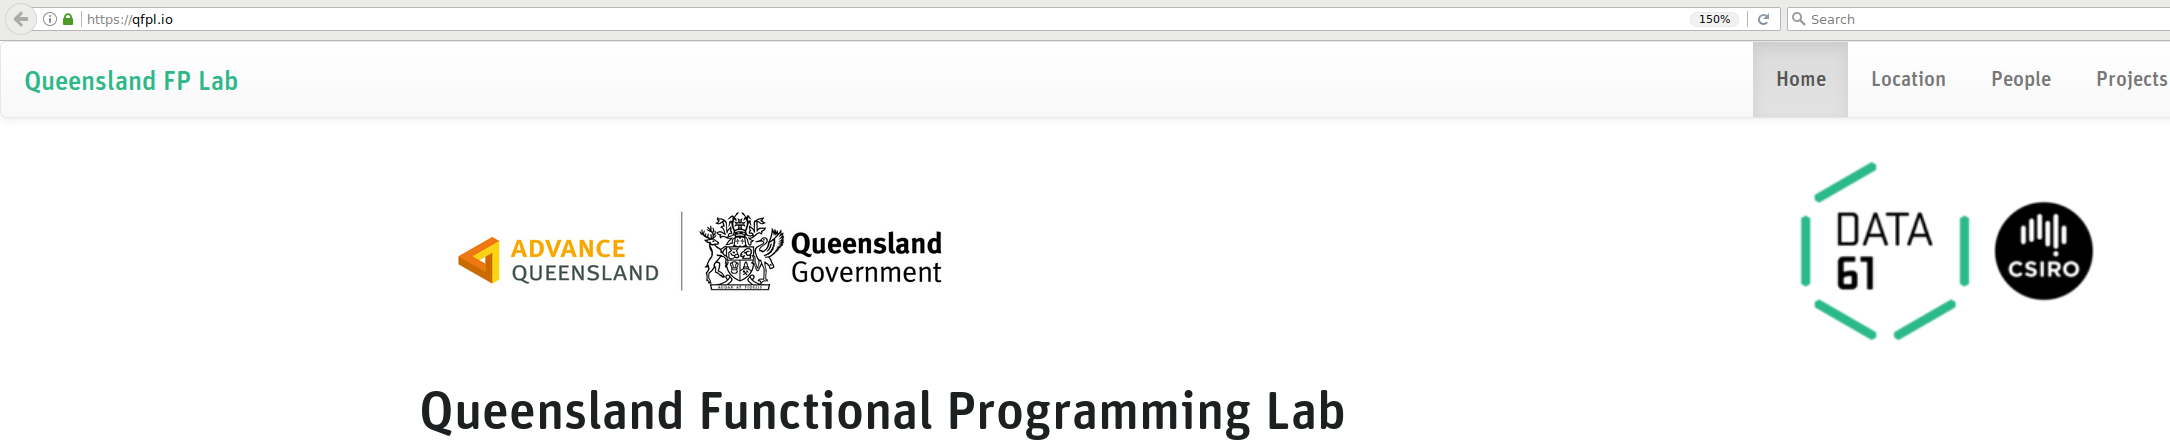
\includegraphics[height=0.24\textheight]{image/qfpl-io.png}
\end{block}
\end{frame}

\begin{frame}
\frametitle{Frequently Asked Questions}
\begin{block}{FAQ}
\begin{itemize}
\item<1-> \textbf{How can I be notified of upcoming FP courses?}

  Subscribe to this mailing list \url{http://notify.qfpl.io/}
\item<2-> \textbf{Do you do non-introductory FP courses?}

  Starting in 2018. Sign up to notifications.
\item<3-> \textbf{Do you do paid professional FP courses?}

  Yes. Contact the QFPL team \href{mailto:contact@qfpl.io}{contact@qfpl.io}
\end{itemize}
\end{block}
\end{frame}

% \begin{frame}
% \begin{center}
% TODO \cite{abbott2005data}
% \end{center}
% \end{frame}

\begin{frame}
\begin{center}
The term zipper is a colloquial that is used to describe n-hole contexts into a data structure; most often \lstinline{n=1}.
\end{center}
\end{frame}

\begin{frame}
\begin{center}
That is, a data structure that has a hole or pointer focussed on a specific element.
\end{center}
\end{frame}

\begin{frame}
\begin{center}
An important property of a zipper is an ability to efficiently traverse to and modify neighbours.
\end{center}
\end{frame}

\begin{frame}
\begin{block}{Loosely speaking}
\begin{center}
Take any data structure and walk to any point (1-hole) on it.
\end{center}
\end{block}
\begin{center}
Now look around you. What do you see?
\end{center}
\end{frame}

\begin{frame}
\begin{block}{For example}
\begin{center}
Here is the list one to ten
\end{center}
\end{block}
\begin{center}
\lstinline{[1,2,3,4,5,6,7,8,9,10]}
\end{center}
\end{frame}

\begin{frame}
\begin{block}{For example}
\begin{center}
Here is a depiction of a physical list one to ten
\end{center}
\end{block}
\begin{center}
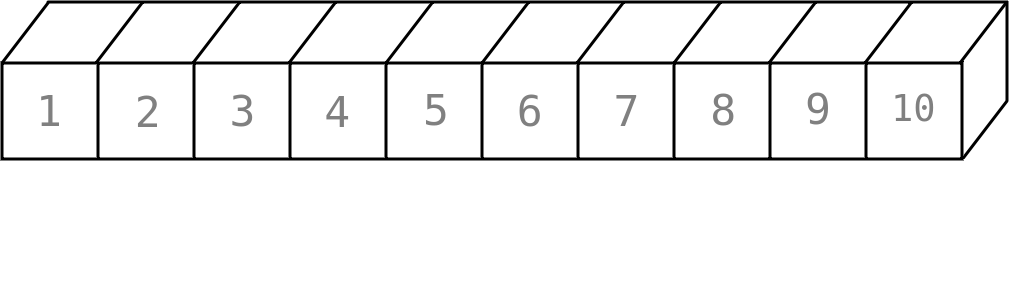
\includegraphics[width=1.25\textheight]{image/list1-10.png}
\end{center}
\end{frame}

\begin{frame}
\begin{block}{For example}
\begin{center}
Let's move to the element containing \lstinline{7}
\end{center}
\end{block}
\begin{center}
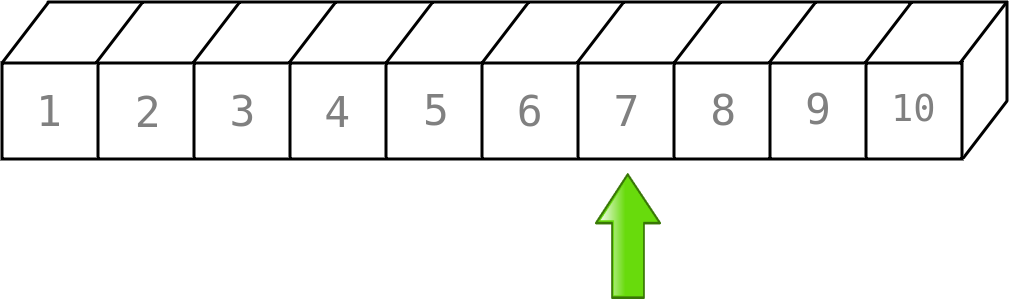
\includegraphics[width=1.25\textheight]{image/list1-10-arrow7.png}
\end{center}
\end{frame}

\begin{frame}
\begin{block}{List zipper}
\begin{center}
and look around us
\end{center}
\end{block}
\begin{center}
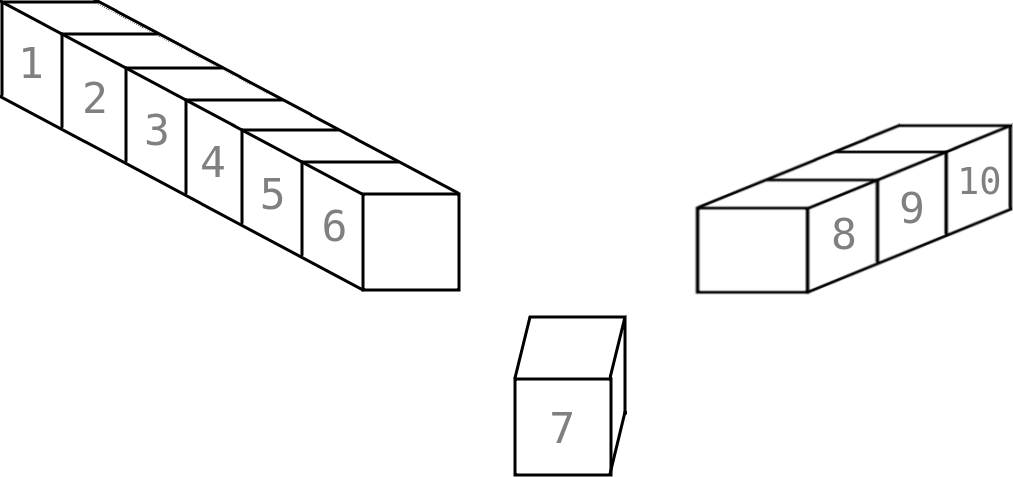
\includegraphics[width=1.25\textheight]{image/listzipper1-10.png}
\end{center}
\begin{center}
\lstinline{([6,5,4,3,2,1], 7, [8,9,10])}
\end{center}
\end{frame}

\begin{frame}
\begin{block}{List zipper}
\begin{center}
and look around us
\end{center}
\end{block}
\begin{center}
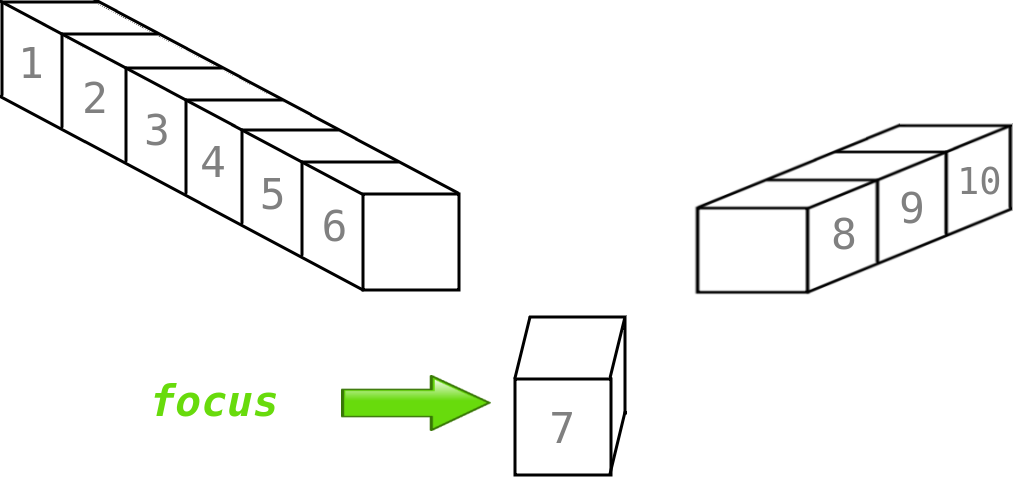
\includegraphics[width=1.25\textheight]{image/listzipper1-10-focus.png}
\end{center}
\begin{center}
\lstinline{([6,5,4,3,2,1], 7, [8,9,10])}
\end{center}
\end{frame}

\begin{frame}[fragile]
\begin{block}{List zipper}
\begin{center}
We can easily move to our neighbours in O(1) time
\end{center}
\end{block}
\begin{center}
\begin{lstlisting}[style=haskell]
listz =
  ([6,5,4,3,2,1], 7, [8,9,10])
  
moveLeft listz =
  ([5,4,3,2,1], 6, [7,8,9,10])
\end{lstlisting}
\end{center}
\end{frame}

\begin{frame}[fragile]
\begin{block}{List zipper}
\begin{center}
The zipper for \lstinline{[a]} is \lstinline{([a], a, [a])}
\end{center}
\end{block}
\begin{center}
\begin{lstlisting}[style=haskell]
data ListZipper a =
  ListZipper [a] a [a]
\end{lstlisting}
\end{center}
\end{frame}

\begin{frame}[fragile]
\begin{block}{List zipper}
\begin{center}
Some useful operations on a list zipper:
\begin{itemize}
  \item \tiny{\lstinline{moveLeft/Right :: ListZipper a -> Maybe (ListZipper a)}}
  \item \tiny{\lstinline{findLeft/Right :: (a -> Bool) -> ListZipper a -> Maybe (ListZipper a)}}
  \item \tiny{\lstinline{modify :: (a -> a) -> ListZipper a -> ListZipper a}}
  \item \tiny{\lstinline{delete :: ListZipper a -> Maybe (ListZipper a)}}
\end{itemize}
\end{center}
\end{block}
\end{frame}

\begin{frame}[fragile]
\begin{block}{Multi-way Tree}
\begin{center}
How about a multi-way tree?
\end{center}
\end{block}
\begin{center}
\begin{lstlisting}[style=haskell]
data Tree a =
  Tree a [Tree a]
\end{lstlisting}
\end{center}
\end{frame}

\begin{frame}[fragile]
\begin{block}{What if we stand on an element and look around?}
\begin{center}
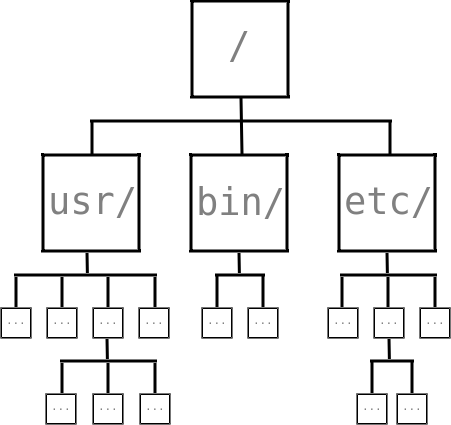
\includegraphics[width=0.60\textheight]{image/rosetree.png}
\end{center}
\end{block}
\end{frame}

\begin{frame}[fragile]
\begin{block}{\lstinline{leftSiblings :: ?}}
\begin{center}
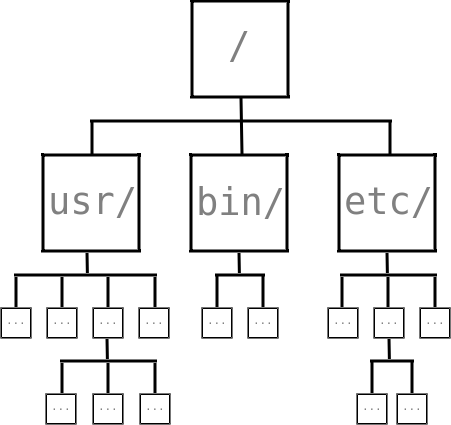
\includegraphics[width=0.60\textheight]{image/rosetree.png}
\end{center}
\end{block}
\end{frame}

\begin{frame}[fragile]
\begin{block}{\lstinline{leftSiblings :: [Tree a]}}
\begin{center}
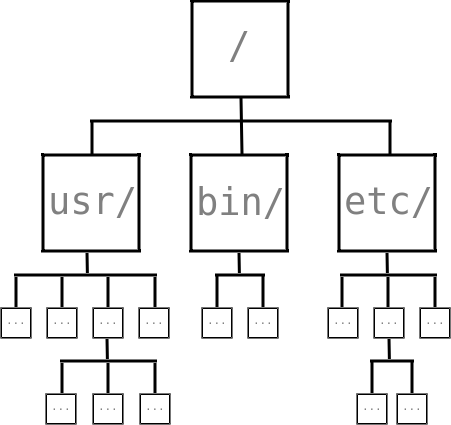
\includegraphics[width=0.60\textheight]{image/rosetree.png}
\end{center}
\end{block}
\end{frame}

\begin{frame}[fragile]
\begin{block}{\lstinline{rightSiblings :: [Tree a]}}
\begin{center}
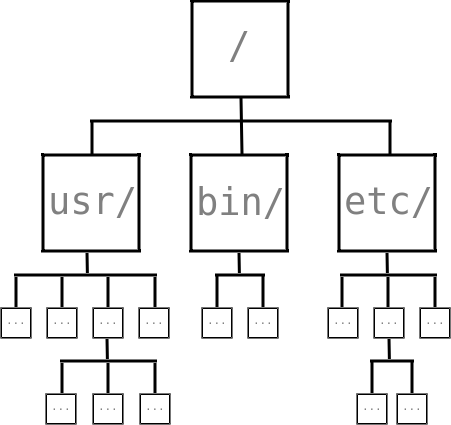
\includegraphics[width=0.60\textheight]{image/rosetree.png}
\end{center}
\end{block}
\end{frame}

\begin{frame}[fragile]
\begin{block}{\lstinline{focus :: ?}}
\begin{center}
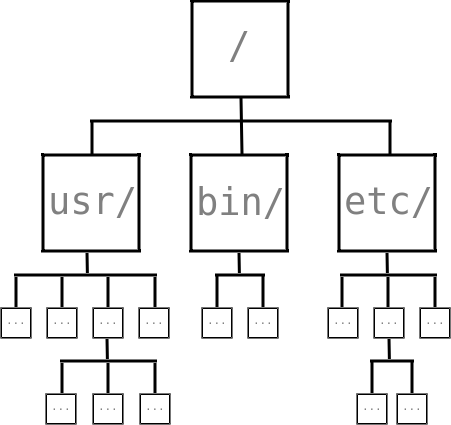
\includegraphics[width=0.60\textheight]{image/rosetree.png}
\end{center}
\end{block}
\end{frame}

\begin{frame}[fragile]
\begin{block}{\lstinline{focus :: a}}
\begin{center}
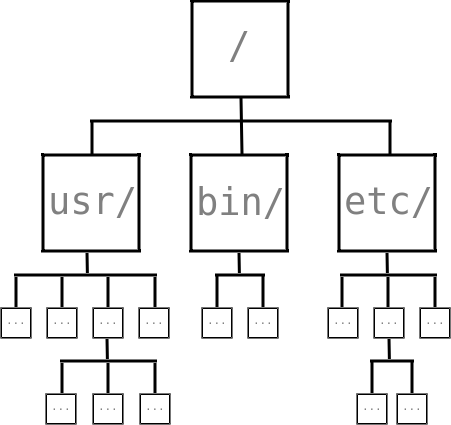
\includegraphics[width=0.60\textheight]{image/rosetree.png}
\end{center}
\end{block}
\end{frame}

\begin{frame}[fragile]
\begin{block}{\lstinline{children :: ?}}
\begin{center}
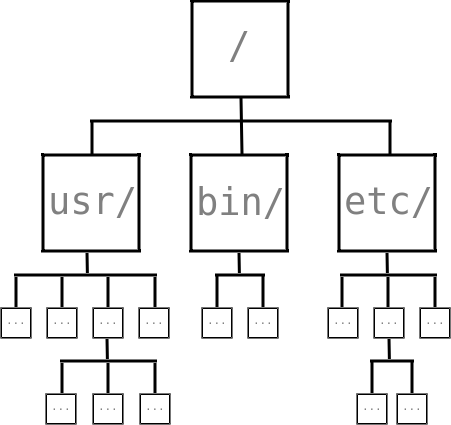
\includegraphics[width=0.60\textheight]{image/rosetree.png}
\end{center}
\end{block}
\end{frame}

\begin{frame}[fragile]
\begin{block}{\lstinline{children :: [Tree a]}}
\begin{center}
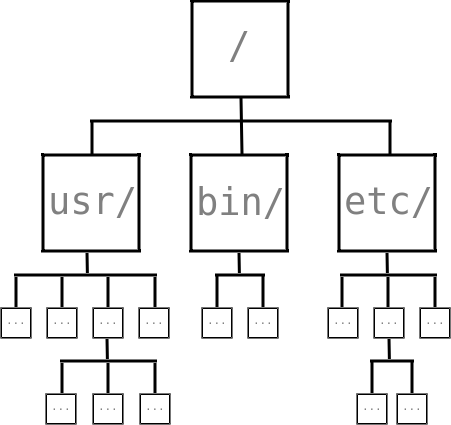
\includegraphics[width=0.60\textheight]{image/rosetree.png}
\end{center}
\end{block}
\end{frame}

\begin{frame}[fragile]
\begin{block}{\lstinline{parents :: ?}}
\begin{center}
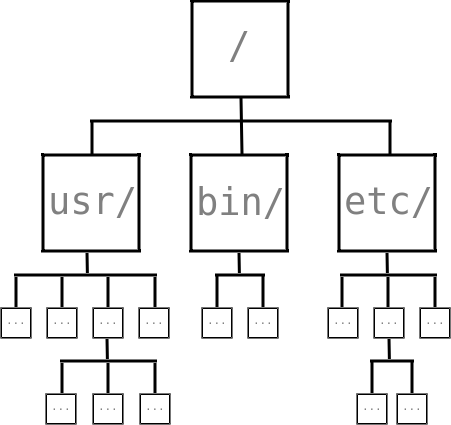
\includegraphics[width=0.60\textheight]{image/rosetree.png}
\end{center}
\end{block}
\end{frame}

\begin{frame}[fragile]
\begin{block}{\lstinline{parents :: [([Tree a], a, [Tree a])]}}
\begin{center}
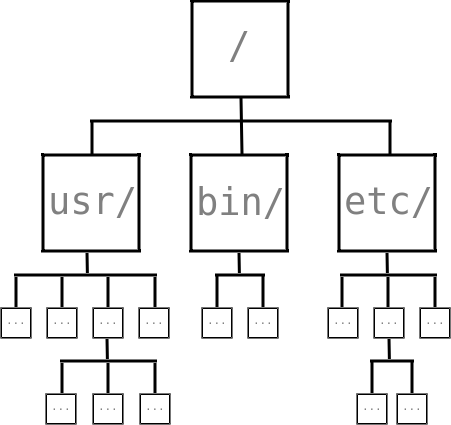
\includegraphics[width=0.60\textheight]{image/rosetree.png}
\end{center}
\end{block}
\end{frame}

\begin{frame}[fragile]
\begin{block}{The zipper for a multi-way tree is}
\begin{lstlisting}[style=haskell]
data TreeZipper a =
  TreeZipper
    [Tree a]                -- left siblings
    [Tree a]                -- right siblings
    a                       -- focus
    [Tree a]                -- children
    ([Tree a], a, [Tree a]) -- parents
\end{lstlisting}
\end{block}
\end{frame}

\begin{frame}[fragile]
\begin{block}{Tree zipper}
\begin{center}
Some useful operations on a tree zipper:
\begin{itemize}
  \item \tiny{\lstinline{moveParent/Child :: TreeZipper a -> Maybe (TreeZipper a)}}
  \item \tiny{\lstinline{moveLeft/Right :: TreeZipper a -> Maybe (TreeZipper a)}}
  \item \tiny{\lstinline{find :: (a -> Bool) -> TreeZipper a -> Maybe (TreeZipper a)}}
  \item \tiny{\lstinline{all :: (a -> Bool) -> TreeZipper a -> Bool}}
  \item \tiny{\lstinline{modify :: (a -> a) -> TreeZipper a -> TreeZipper a}}
  \item \tiny{\lstinline{modifyTree :: (Tree a -> Tree a) -> TreeZipper a -> TreeZipper a}}
  \item \tiny{\lstinline{insertSiblingLeft/Right :: Tree a -> TreeZipper a -> TreeZipper a}}
\end{itemize}
\end{center}
\end{block}
\end{frame}

\begin{frame}[fragile]
\begin{block}{Other zippers}
\begin{center}
Some other data structures have useful zippers:
\begin{itemize}
  \item JSON
  \item CSV
  \item ASN.1
  \item text editors
  \item Pilot logbook
  \item \emph{many more!}
\end{itemize}
\end{center}
\end{block}
\end{frame}

\begin{frame}
\begin{center}
Speaking of useful operations\ldots
\end{center}
\end{frame}

\begin{frame}
\begin{block}{Comonad is}
Any functor \lstinline{F} supporting:
\begin{center}
\begin{itemize}
  \item<1-> \lstinline{extract :: F a -> a}
  \item<2-> \lstinline{duplicate :: F a -> F (F a)}
  \item<3-> \emph{satisfying laws of identity and associativity}
\end{itemize}
\end{center}
\end{block}
\end{frame}

\begin{frame}
\begin{center}
Does a \lstinline{ListZipper} satisfy the requirements for a comonad?
\end{center}
\end{frame}

\begin{frame}[fragile]
\begin{block}{Yes}
\begin{center}
\begin{lstlisting}[style=haskell]
fmap :: (a -> b) -> ListZipper a -> ListZipper b
extract :: ListZipper x -> x
duplicate :: ListZipper w -> ListZipper (ListZipper w)
\end{lstlisting}
\end{center}
\end{block}
\end{frame}

\begin{frame}
\begin{center}
What about a \lstinline{TreeZipper}?
\end{center}
\end{frame}

\begin{frame}[fragile]
\begin{block}{Yes}
\begin{center}
\begin{lstlisting}[style=haskell]
fmap :: (a -> b) -> TreeZipper a -> TreeZipper b
extract :: TreeZipper x -> x
duplicate :: TreeZipper w -> TreeZipper (TreeZipper w)
\end{lstlisting}
\end{center}
\end{block}
\end{frame}

\begin{frame}[fragile]
\begin{block}{Actually}
\begin{center}
\textbf{All} zippers are comonads \emph{(Uustalu, 2005)}
\end{center}
\end{block}
\end{frame}

\begin{frame}[fragile]
\begin{block}{Here is a utility function}
\begin{center}
\begin{lstlisting}[style=haskell]
-- Do any (max: 2) adjacent focii of the list zipper
-- satisfy the given predicate?
adjacentFociiSatisfy ::
  (a -> Bool)
  -> ListZipper a
  -> Bool
adjacentFociiSatisfy p z =
  let mvs k = any p (focus <$> k z)
  in  mvs moveLeft || mvs moveRight
\end{lstlisting}
\end{center}
\end{block}
\end{frame}

\begin{frame}[fragile]
\begin{block}{Requirement}
\begin{center}
Find all zippers with a focus adjacent to a given value
\end{center}
\end{block}
\end{frame}

\begin{frame}[fragile]
\begin{block}{Find all zippers with a focus adjacent to a given value}
\begin{itemize}
  \item<1-> \lstinline{duplicate}

            we now have \lstinline{ListZipper (ListZipper a)}
  \item<2-> \lstinline{toList}

            we now have \lstinline{[ListZipper a]}
  \item<3-> \lstinline{filter} with \lstinline{adjacentFociiSatisfy}

            we still have \lstinline{[ListZipper a]}
\end{itemize}
\end{block}
\end{frame}

\begin{frame}[fragile]
\begin{block}{\lstinline{allWithAdjacent}}
\begin{center}
\begin{lstlisting}[style=haskell]
allWithAdjacent ::
  Eq a =>
  a
  -> ListZipper a
  -> [ListZipper a]
allWithAdjacent n =
  filter (adjacentFociiSatisfy (==n)) . toList . duplicate
\end{lstlisting}
\end{center}
\end{block}
\end{frame}

\begin{frame}[fragile]
\begin{block}{\lstinline{allWithAdjacent}}
\begin{center}
\begin{lstlisting}[style=haskell]
> allWithAdjacent 3 (ListZipper [3,2,1] 4 [5..10])
[
  ListZipper {
    lefts = [1]
  , focus = 2
  , rights = [3,4,5,6,7,8,9,10]
  }
, ListZipper {
    lefts = [3,2,1]
  , focus = 4
  , rights = [5,6,7,8,9,10]
  }
]
\end{lstlisting}
\end{center}
\end{block}
\end{frame}

\begin{frame}[fragile]
\begin{block}{\lstinline{allWithAdjacent}}
\begin{center}
\begin{lstlisting}[style=haskell]
> allWithAdjacent 3 (ListZipper [3,2,1] 4 [7,2,6,3])
[
  ListZipper {
    lefts = [1]
  , focus = 2
  , rights = [3,4,7,2,6,3]
  }
, ListZipper {
    lefts = [3,2,1]
  , focus = 4
  , rights = [7,2,6,3]
  }
, ListZipper {
    lefts = [2,7,4,3,2,1]
  , focus = 6
  , rights = [3]
  }
]
\end{lstlisting}
\end{center}
\end{block}
\end{frame}

\begin{frame}
\begin{center}
Who's wanted that in their text editor before?
\end{center}
\end{frame}

\begin{frame}
\begin{center}
What were you editing? JSON? Your pilot logbook?
\end{center}
\end{frame}

\begin{frame}
\begin{center}
What about \textbf{a programming language}?
\end{center}
\end{frame}

% \begin{frame}
% \begin{center}
% I'll leave \lstinline{TreeZipper} comonad operations to your imagination
% \end{center}
% \end{frame}

\begin{frame}
\begin{block}{other uses of zippers}
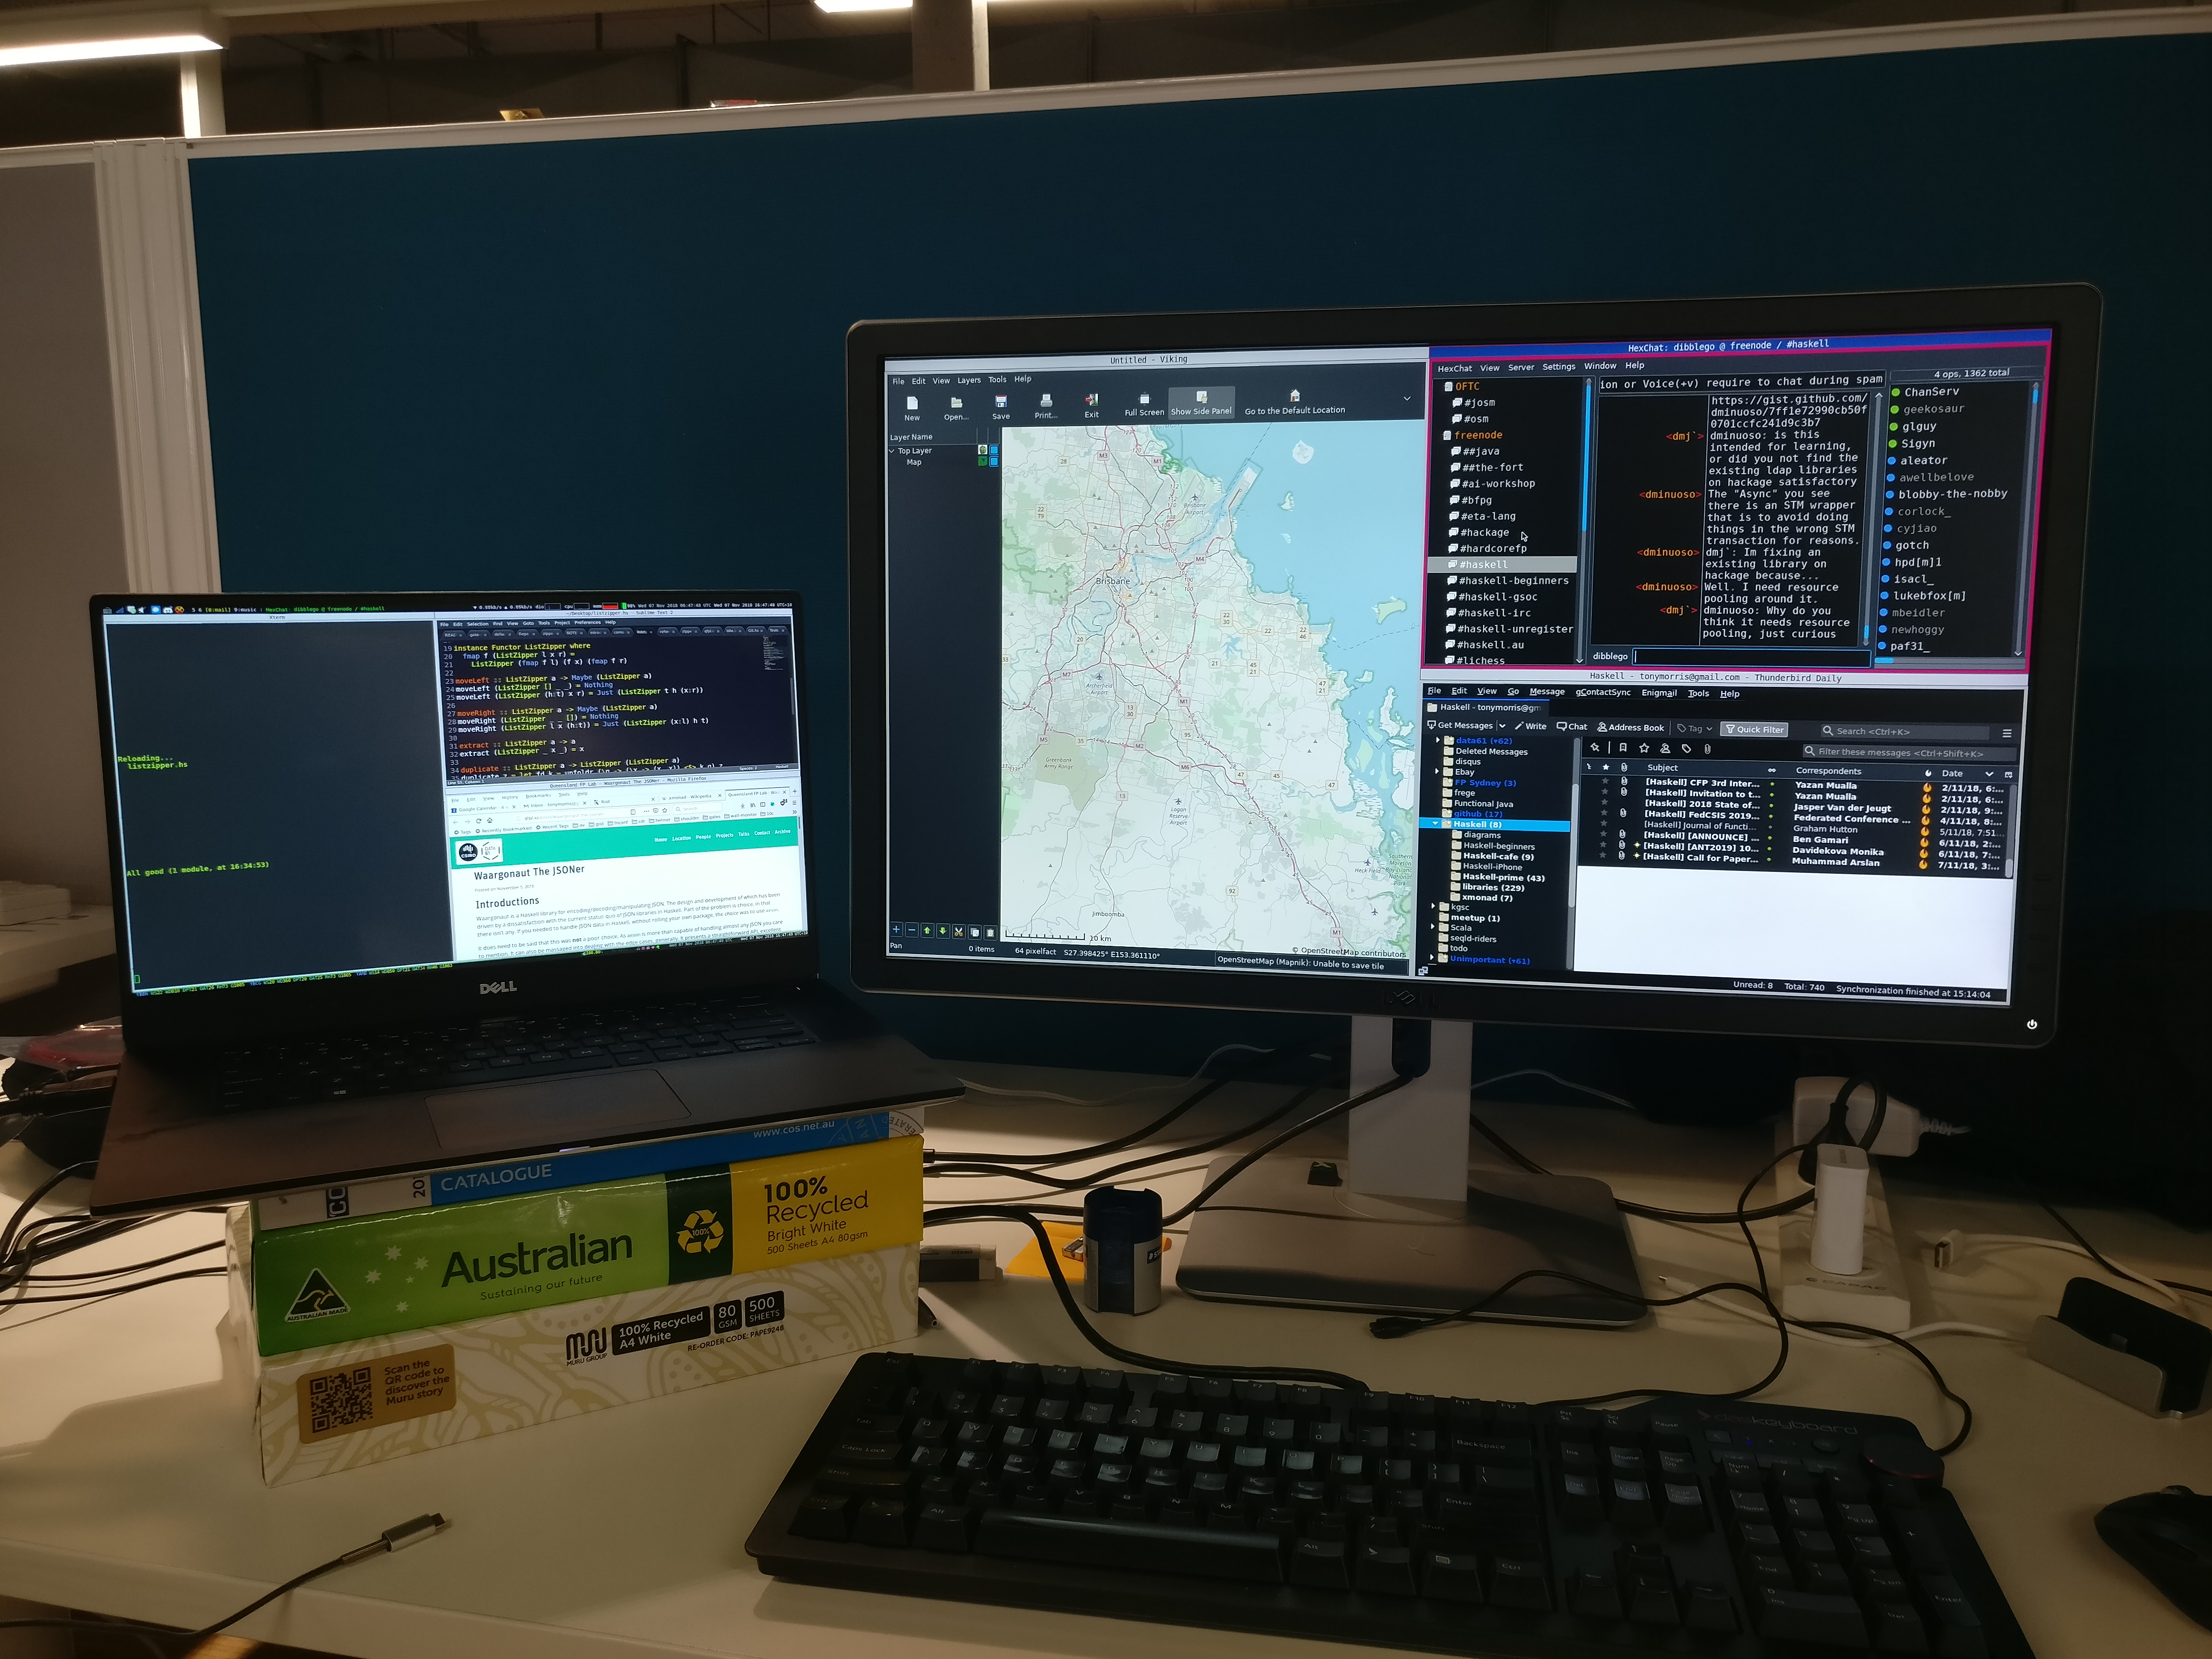
\includegraphics[width=1.00\textheight]{image/xmonad.jpg}
\end{block}
\end{frame}

\begin{frame}
\begin{block}{OK, but\ldots}
Why zipper?

If I wanted to modify the element of a tree, why wouldn't I use a lens (or traversal)?
\end{block}
\end{frame}

\begin{frame}[fragile]
\begin{block}{OK, but\ldots}
\begin{lstlisting}[style=haskell]
immediateChildren :: Traversal (Tree a) (Tree a)
focus :: Lens (Tree a) a
\end{lstlisting}
\end{block}
\end{frame}

\begin{frame}
\begin{block}{Zipper vs Lens}
\begin{center}
While lens gives you nice compositional properties, zipper does \emph{context-dependent} updates
\end{center}
\end{block}
\end{frame}

\begin{frame}
\begin{block}{Zipper vs Lens}
\begin{center}
\begin{itemize}
  \item \textbf{lens} \begin{quote}view one hole in a data structure, then operate on it\end{quote}
  \item \textbf{traversal} \begin{quote}view many holes in a data structure, then operate on it\end{quote}
  \item \textbf{zipper} \begin{quote}view one hole in a data structure, then \textbf{depend} on it to move efficiently to another hole (and so on)\end{quote}
\end{itemize}
\end{center}
\end{block}
\end{frame}

\begin{frame}
\begin{block}{Zipper vs Lens}
\begin{center}
\begin{itemize}
  \item \textbf{lens} \begin{quote}view and operate on \lstinline{y} in \lstinline{(x, y, z)}\end{quote}
  \item \textbf{traversal} \begin{quote}view and operate on all of the \lstinline{y} in \lstinline{(x, y, z, y, [y])}\end{quote}
  \item \textbf{zipper} \begin{quote}view and operate on a specific \lstinline{y} in \lstinline{(y, y, y)} and depending on the operation outcome, move to a different \lstinline{y} (and so on)\end{quote}
\end{itemize}
\end{center}
\end{block}
\end{frame}

\begin{frame}
\begin{block}{Algebra}
Algebraic Data Types can be thought of in terms of regular algebraic equations
\end{block}
\end{frame}

\begin{frame}
\begin{block}{Some examples include}
\begin{itemize}
  \item \textbf{sum types}

        \lstinline{Either A B} or ``A or B'' corresponds to the equation \lstinline{A + B}
  \item \textbf{product types}

        \lstinline{(A, B)} or ``A and B'' corresponds to the equation \lstinline{A * B}
  \item \textbf{exponentiation}

        \lstinline{A -> B} corresponds to the equation \lstinline{B}\textsuperscript{\lstinline{A}}
  \item \textbf{unit}

        given \lstinline{data Unit = Unit},

        the \lstinline{Unit} data type corresponds to the value \lstinline{1}
  \item \textbf{void}

        given \lstinline{data Void},

        the \lstinline{Void} data type corresponds to the value \lstinline{0}
\end{itemize}
\end{block}
\end{frame}

\begin{frame}[fragile]
\begin{block}{Let's look at \lstinline{Bool}}
\begin{lstlisting}
data Bool = True | False
\end{lstlisting}
\begin{itemize}
  \item<1-> The \lstinline{True} constructor has no arguments, which is equivalent to carrying \lstinline{Unit}
  \item<1-> The \lstinline{False} constructor has no arguments, which is equivalent to carrying \lstinline{Unit}
  \item<2-> The whole data type carries \lstinline{1} or \lstinline{1}
  \item<2-> \lstinline{Bool ~ 1 + 1 ~ 2}
\end{itemize}
\end{block}
\end{frame}

\begin{frame}[fragile]
\begin{block}{How about \lstinline{Maybe a}}
\begin{lstlisting}
data Maybe a = Nothing | Just a
\end{lstlisting}
\begin{itemize}
  \item<1-> The \lstinline{Nothing} constructor has no arguments, which is equivalent to carrying \lstinline{Unit}
  \item<1-> The \lstinline{Just} constructor has an argument \lstinline{a}
  \item<2-> The whole data type carries \lstinline{1} or \lstinline{a}
  \item<2-> \lstinline{Maybe a ~ 1 + a}
\end{itemize}
\end{block}
\end{frame}

\begin{frame}[fragile]
\begin{block}{Another one \lstinline{Either Void a}}
\begin{lstlisting}
\end{lstlisting}
\begin{itemize}
  \item<1-> The \lstinline{Left} constructor carries \lstinline{0}
  \item<1-> The \lstinline{Right} constructor has an argument \lstinline{a}
  \item<2-> The whole data type carries \lstinline{0} or \lstinline{a}
  \item<2-> \lstinline{Either Void a ~ 0 + a ~ a}
\end{itemize}
\end{block}
\end{frame}

\begin{frame}[fragile]
\begin{block}{and another \lstinline{(Void, a)}}
\begin{lstlisting}
\end{lstlisting}
\begin{itemize}
  \item<1-> The whole data type carries \lstinline{0} and \lstinline{a}
  \item<2-> \lstinline{(Void, a) ~ 0 * a ~ 0}
\end{itemize}
\end{block}
\end{frame}

\begin{frame}
\begin{block}{lost of \lstinline{Bool}}
\begin{itemize}
  \item<1-> \lstinline{(Bool, Bool)}
  \item<1-> \lstinline{Either Bool Bool}
  \item<1-> \lstinline{Bool -> Bool}
  \item<2-> \lstinline{2 * 2}
  \item<2-> \lstinline{2 + 2}
  \item<2-> \lstinline{2}\textsuperscript{\lstinline{2}}
  \item<3-> These are all \lstinline{4}
\end{itemize}
\end{block}
\end{frame}

\begin{frame}
\begin{block}{Inhabitants}
The resulting algebraic equation gives us the number of \emph{inhabitants}.

Or, the number of values with that type.
\end{block}
\end{frame}

\begin{frame}
\begin{block}{Inhabitants}
\begin{itemize}
  \item<1-> \lstinline{Maybe (Bool -> Maybe Bool)}
  \item<1-> has \lstinline{1 + (1 + 2)}\textsuperscript{\lstinline{3}} inhabitants
  \item<1-> \lstinline{10} inhabitants
  \item<2-> \scriptsize{\lstinline{(Either Bool (Maybe Bool), Bool, (Unit, Bool), Either Void Bool)}}
  \item<2-> has \lstinline{(2 + (1 + 2)) * 2 * (1 * 2) * (0 + 2)} inhabitants
  \item<2-> \lstinline{40}
\end{itemize}
\end{block}
\end{frame}

\begin{frame}
\begin{block}{Algebraically}
\begin{center}
What is \lstinline{[a]}?
\end{center}
\end{block}
\end{frame}

\begin{frame}
\begin{block}{Lists}
\begin{itemize}
  \item<1-> \lstinline{[a]} is either zero \lstinline{a} or one \lstinline{a} or two \lstinline{a} \ldots
  \item<2-> \lstinline{a}\textsuperscript{\lstinline{0}} \lstinline{+ a}\textsuperscript{\lstinline{1}} \lstinline{+ a}\textsuperscript{\lstinline{2}} \ldots
  \item<3-> using algebraic rules, this simplifies to \lstinline{1 + a * [a]}
  \item<3-> \lstinline{1} or \lstinline{(a and [a])}
  \item<3-> The \lstinline{[]} \emph{(carrying \lstinline{Unit})} or \lstinline{(:)} constructor
\end{itemize}
\end{block}
\end{frame}

\begin{frame}
\begin{center}
Here is a data type:

\lstinline{Either x (x, x)}
\end{center}
\end{frame}


\begin{frame}
\begin{center}
Algebraically:

\lstinline{x + (x * x)}
\end{center}
\end{frame}


\begin{frame}
\begin{center}
Differentiate

$\frac{\partial}{\partial x}$ \lstinline{(x + (x * x))}
\end{center}
\end{frame}


\begin{frame}
\begin{center}
$\frac{\partial}{\partial x}$ \lstinline{(x + (x * x))}

\tiny{\emph{(sum rule)}}\normalsize{}

\lstinline{=} $\frac{\partial}{\partial x}$ \lstinline{(x +} $\frac{\partial}{\partial x}$ \lstinline{(x * x))}

\tiny{\emph{(power rule, line rule)}}\normalsize{}

\lstinline{= 1 + (2 * x)}

\par\noindent\rule{\textwidth}{0.4pt}

\lstinline{= Maybe (x, x)}
\end{center}
\end{frame}


\begin{frame}
\begin{block}{$\therefore$}
\begin{center}
$\frac{\partial}{\partial x}$ \lstinline{Either x (x, x)}

\par\noindent\rule{\textwidth}{0.4pt}

\lstinline{= Maybe (x, x)}
\end{center}
\end{block}
\end{frame}


\begin{frame}
\begin{block}{$\frac{\partial}{\partial x}$ \lstinline{Either x (x, x)}}
\begin{center}
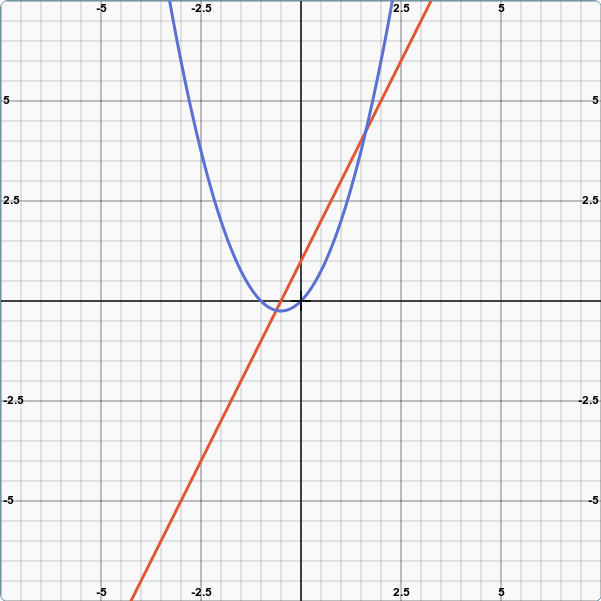
\includegraphics[width=0.75\textheight]{image/derivative_x_plus_x_times_x.png}
\end{center}
\end{block}
\end{frame}


\begin{frame}
\begin{center}
We'll do another one

\lstinline{(Either x x, Either x x)}
\end{center}
\end{frame}


\begin{frame}
\begin{center}
Algebraically:

\lstinline{(x + x) * (x + x)}
\end{center}
\end{frame}


\begin{frame}
\begin{center}
Differentiate

$\frac{\partial}{\partial x}$ \lstinline{((x + x) * (x + x))}
\end{center}
\end{frame}


\begin{frame}
\begin{center}
$\frac{\partial}{\partial x}$ \lstinline{((x + x) * (x + x))}

\lstinline{=} $\frac{\partial}{\partial x}$ \lstinline{4 * x}\textsuperscript{\lstinline{2}}

\tiny{\emph{(power rule)}}\normalsize{}

\lstinline{= 4 *} $\frac{\partial}{\partial x}$ \lstinline{x}\textsuperscript{\lstinline{2}}

\tiny{\emph{(power rule)}}\normalsize{}

\lstinline{= 4 * 2 * x}

\par\noindent\rule{\textwidth}{0.4pt}

\lstinline{= 8 * x}
\end{center}
\end{frame}


\begin{frame}
\begin{block}{$\therefore$}
\begin{center}
$\frac{\partial}{\partial x}$ \lstinline{(Either x x, Either x x)}

\par\noindent\rule{\textwidth}{0.4pt}

\lstinline{= (x, x, x, x, x, x, x, x)}
\end{center}
\end{block}
\end{frame}


\begin{frame}
\begin{center}
A simpler one

\lstinline{(x, x, x)}
\end{center}
\end{frame}


\begin{frame}
\begin{center}
Algebraically:

\lstinline{x * x * x}
\end{center}
\end{frame}


\begin{frame}
\begin{center}
Differentiate

$\frac{\partial}{\partial x}$ \lstinline{x * x * x}
\end{center}
\end{frame}


\begin{frame}
\begin{center}
$\frac{\partial}{\partial x}$ \lstinline{x * x * x}

\lstinline{=} $\frac{\partial}{\partial x}$ \lstinline{x}\textsuperscript{\lstinline{3}}

\tiny{\emph{(power rule)}}\normalsize{}

\lstinline{= 3 *} \lstinline{x}\textsuperscript{\lstinline{2}}
\end{center}
\end{frame}


\begin{frame}
\begin{block}{$\therefore$}
\begin{center}
$\frac{\partial}{\partial x}$ \lstinline{(x, x, x)}

\par\noindent\rule{\textwidth}{0.4pt}

\lstinline{= (Maybe Bool, x, x)}
\end{center}
\end{block}
\end{frame}


\begin{frame}
\begin{center}

\includegraphics[width=0.3\textheight]{image/crosseyed-blank.png}
\end{center}
\begin{block}{Summary}
\begin{itemize}
  \item \scriptsize{$\frac{\partial}{\partial x}$ \lstinline{Either x (x, x) = Maybe (x, x)}}
  \item \scriptsize{$\frac{\partial}{\partial x}$ \lstinline{(Either x x, Either x x) = (x, x, x, x, x, x, x, x)}}
  \item \scriptsize{$\frac{\partial}{\partial x}$ \lstinline{(x, x, x) = (Maybe Bool, x, x)}}
\end{itemize}
\end{block}
\end{frame}


\begin{frame}
\begin{block}{Insight}
\begin{center}
  The derivative of \emph{any} data structure, \textbf{is its zipper!}\cite{abbott2005data} \footnote{\emph{without the 1-hole context value}}
\end{center}
\end{block}
\end{frame}


\begin{frame}
\begin{center}

\includegraphics[width=0.3\textheight]{image/crosseyed.png}
\end{center}
\begin{block}{Let's stare}
\begin{itemize}
  \item \scriptsize{$\frac{\partial}{\partial x}$ \lstinline{Either x (x, x) = Maybe (x, x)}}
  \item \scriptsize{$\frac{\partial}{\partial x}$ \lstinline{(Either x x, Either x x) = (x, x, x, x, x, x, x, x)}}
  \item \scriptsize{$\frac{\partial}{\partial x}$ \lstinline{(x, x, x) = (Maybe Bool, x, x)}}
\end{itemize}
\end{block}
\end{frame}

\begin{frame}
\begin{block}{Let's do list \tiny{you know you want to}}
\lstinline{List a = 1 + a + a}\textsuperscript{\lstinline{2}} \lstinline{+ a}\textsuperscript{\lstinline{3}} \lstinline{+} \ldots
\end{block}
\end{frame}

\begin{frame}{List}

\lstinline{List a = 1 + a + a}\textsuperscript{\lstinline{2}} \lstinline{+ a}\textsuperscript{\lstinline{3}} \lstinline{+} \ldots

\par\noindent\rule{\textwidth}{0.4pt}

\lstinline{let K a = a + a}\textsuperscript{\lstinline{2}} \lstinline{+ a}\textsuperscript{\lstinline{3}} \lstinline{+} \ldots

\lstinline{List a = 1 + K a}

\emph{\tiny{multiply list by \lstinline{a}}}

\lstinline{K a = a * List a}

\par\noindent\rule{\textwidth}{0.4pt}

{$\therefore$} List a = 1 + a * List a

\emph{\tiny{this makes sense if we think of \lstinline{List} in terms of its constructors}}

\end{frame}


\begin{frame}{List}

\lstinline{List a = 1 + a * List a}

\par\noindent\rule{\textwidth}{0.4pt}

\emph{\tiny{subtract \lstinline{(a * List a)} both sides}}

\lstinline{List a - (a * List a) = 1}

\emph{\tiny{multiply \lstinline{List a} by \lstinline{1}}}

\lstinline{(1 * List a) - (a * List a) = 1}

\emph{\tiny{apply distributive law of multiplication}}

\lstinline{List a * (1 - a) = 1}

\emph{\tiny{divide both sides by \lstinline{1 - a}}}

\lstinline{List a = 1 / (1 - a)}

\par\noindent\rule{\textwidth}{0.4pt}

\emph{\tiny{apply exponent rule}}

{$\therefore$} \lstinline{List a = (1 - a)}\textsuperscript{\lstinline{-1}}

\end{frame}


\begin{frame}{List}

\lstinline{List a = (1 - a)}\textsuperscript{\lstinline{-1}}

\par\noindent\rule{\textwidth}{0.4pt}

\lstinline{let u = 1 - a}

\emph{\tiny{apply chain rule}}

$\frac{\partial}{\partial a}$ {\lstinline{(1 - a)}\textsuperscript{\lstinline{-1}}} \lstinline{=} $\frac{\partial}{\partial u}$ {\lstinline{u}\textsuperscript{\lstinline{-1}}} \lstinline{*} $\frac{\partial}{\partial a}$ \lstinline{1 - a}

\emph{\tiny{differentiate \lstinline{u}\textsuperscript{\lstinline{-1}}}}

$\frac{\partial}{\partial u}$ \lstinline{u}\textsuperscript{\lstinline{-1}} \lstinline{=} \lstinline{-1 / u}\textsuperscript{\lstinline{2}}

\emph{\tiny{differentiate \lstinline{1 - a}}}

$\frac{\partial}{\partial a}$ \lstinline{1 - a} \lstinline{= -1} 

\par\noindent\rule{\textwidth}{0.4pt}

{$\therefore$} $\frac{\partial}{\partial a}$ {\lstinline{(1 - a)}\textsuperscript{\lstinline{-1}}} \lstinline{=} \lstinline{(-1 / u}\textsuperscript{\lstinline{2}}\lstinline{) * -1}

\end{frame}


\begin{frame}{List}

$\frac{\partial}{\partial a}$ {\lstinline{(1 - a)}\textsuperscript{\lstinline{-1}}} \lstinline{=} \lstinline{(-1 / u}\textsuperscript{\lstinline{2}}\lstinline{) * -1}

\par\noindent\rule{\textwidth}{0.4pt}

\emph{\tiny{substitute back \lstinline{u = 1 - a}}}

$\frac{\partial}{\partial a}$ {\lstinline{(1 - a)}\textsuperscript{\lstinline{-1}}} \lstinline{=} \lstinline{(-1 / (1 - a)}\textsuperscript{\lstinline{2}}\lstinline{) * -1}

\emph{\tiny{simplify by multiplying right side by \lstinline{-1}}}

$\frac{\partial}{\partial a}$ {\lstinline{(1 - a)}\textsuperscript{\lstinline{-1}}} \lstinline{=} \lstinline{1 / (1 - a)}\textsuperscript{\lstinline{2}}

\emph{\tiny{apply exponent rule}}

$\frac{\partial}{\partial a}$ {\lstinline{(1 - a)}\textsuperscript{\lstinline{-1}}} \lstinline{=} \lstinline{(1 / 1 - a)}\textsuperscript{\lstinline{2}}

$\frac{\partial}{\partial a}$ {\lstinline{(1 - a)}\textsuperscript{\lstinline{-1}}} \lstinline{=} \lstinline{((1 - a)}\textsuperscript{\lstinline{-1}}\lstinline{)}\textsuperscript{\lstinline{2}}

\par\noindent\rule{\textwidth}{0.4pt}

{$\therefore$} The derivative of a \lstinline{List} is a pair of \lstinline{List}

\end{frame}


\begin{frame}[fragile]
\begin{block}{List derivative}
\begin{lstlisting}[style=haskell]
-- 1 + (a * List a)
List a ~ Nil | Cons a (List a)

-- (1 + (a * List a)) * (1   + (a * List a))
ListDerivative ~ (List a, List a)

-- add the hole back to the derivative
-- (1 + (a * List a)) * a * (1   + (a * List a))
ListZipper ~ (List a, a, List a)
\end{lstlisting}
\end{block}
\end{frame}


\begin{frame}
\begin{center}
\lstinline{data ListZipper a = ListZipper [a] a [a]}
\end{center}

\vspace{1cm}

\begin{center}

\includegraphics[width=0.3\textheight]{image/crosseyed-swirl.png}
\end{center}

\begin{center}
I shall not rob the reader of the fun task of differentiating \lstinline{Tree}

\lstinline{data Tree a = Tree a [Tree a]}

\end{center}

\end{frame}

\begin{frame}
\begin{center}
Thanks!
\end{center}
\end{frame}

\begin{frame}
\frametitle{References}

\bibliographystyle{amsalpha}
\bibliography{zippers}

\end{frame}


\end{document}
